%%This is a very basic article template.
%%There is just one section and two subsections.
%%This is a very basic article template.
%%There is just one section and two subsections.
\documentclass[a4paper,11pt,oneside,brazilian]{article}

\usepackage[utf8]{inputenx}
\usepackage[brazilian]{babel}
\usepackage{graphicx}
\usepackage{float}
\usepackage{textgreek}
\usepackage{mathtools}
\usepackage{enumerate}
\usepackage{xfrac}

\usepackage{multicol}

\usepackage{pgf,tikz}
\usepackage{pgfplots}
\usetikzlibrary{arrows}

\newcommand{\degre}{\ensuremath{^\circ}}
\newcommand{\bfig}{\begin{figure}[!h]\centering}
\newcommand{\efig}{\end{figure}}
\renewcommand{\thesection}{\Roman{section}} 


\definecolor{zzttqq}{rgb}{0.6,0.2,0}
\definecolor{xdxdff}{rgb}{0.49,0.49,1}
\definecolor{qqqqff}{rgb}{0,0,1}
\definecolor{cqcqcq}{rgb}{0.75,0.75,0.75}
\definecolor{uuuuuu}{rgb}{0.27,0.27,0.27}
\definecolor{uququq}{rgb}{0.25,0.25,0.25}
\definecolor{qqwuqq}{rgb}{0.0,0.39215686274509803,0.0}
\definecolor{ffqqqq}{rgb}{1.0,0.0,0.0}
\definecolor{ffffff}{rgb}{1,1,1}
\definecolor{qqqqff}{rgb}{0,0,1}

 \pgfplotsset{compat=1.9}
\begin{document}

\title{Exercícios de Prática e Lógica}
\author{Prof. Eduardo Elael}
\date{Lista ENEM - PVNC 2014}
\maketitle


\begin{flushright}
  \emph{Data da realização:} 13/out/2014
\end{flushright}

\section{Matemática}
\begin{enumerate}[{R}1]
 
  \item Um cubo é lascado em um de seus vértices. Na figura a lasca se encontra
  em azul, e é formada pelo tetraedro de vértices F,I,J e K, sendo I, J e K
  pontos médios de suas respectivas arestas. O percentual de volume que o cubo
  perdeu ao ser lascado é de, aproximadamente:

  \nopagebreak[4]
  \begin{multicols}{2}
  \begin{enumerate}[a)]
    \item $2\%$
    \item $4\%$
    \item $13\%$
    \item $15\%$
    \item $23\%$
  \end{enumerate}
  
	\begin{figure}[H]
	 \centering
	 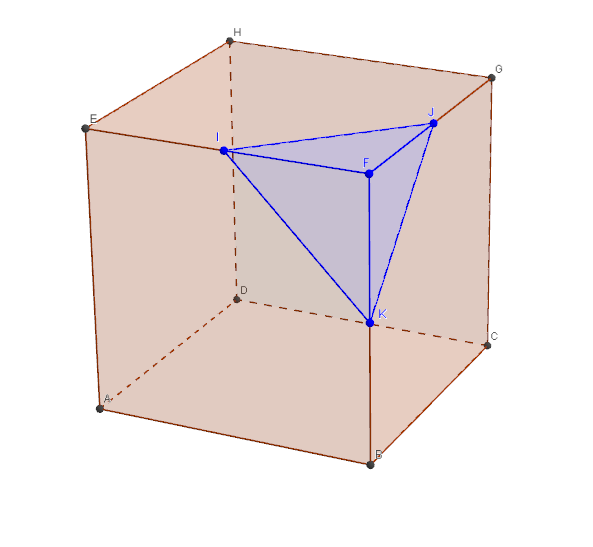
\includegraphics[width=1\columnwidth]{cube.png}
	 \label{fig:cube}
	\end{figure}
  \end{multicols}
  %\nopagebreak[4]
  \pagebreak[4]
  \item Dado um cone reto e a maior esfera que pode ser inscrita nesse cone. Com
  qual desses conjuntos de informações \textbf{não} é possível descobrir a altura do cone:
  

  \begin{multicols}{2}
  \begin{enumerate}[a)]
    \item O ângulo $\hat{ABC}$ do vértice do cone e o raio da esfera.
    \item O volume da cone e o raio da esfera.
    \item O volume da esfera e o raio da base do cone.
    \item A área da base do cone e a área da superfície lateral do cone.
  \end{enumerate}
  
	\begin{figure}[H]
	 \centering
	 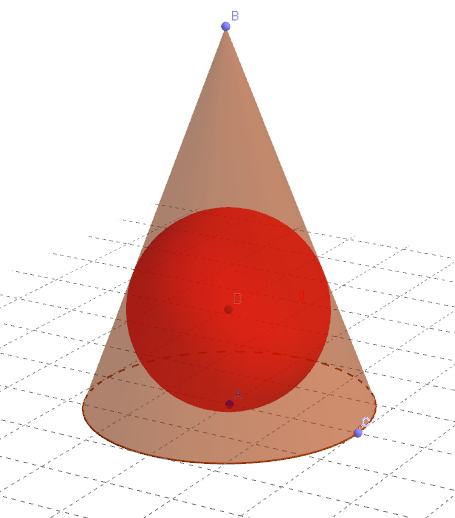
\includegraphics[width=1\columnwidth]{conesphere.png}
	 \label{fig:cube}
	\end{figure}
  \end{multicols}
	 
		
  %\pagebreak[4]
  \item Calcular a área da região DEML na interseção entre dois setores
  circulares é possível fazendo uso das seguintes informações:

  \nopagebreak[4]
  \begin{multicols}{2}
  
  \begin{enumerate}[a)]
    \item Ângulo $\alpha$ e comprimento do segmento EM
    \item Comprimento dos arcos ML e DE
    \item Comprimento do raio interno AM e do segmento ME
    \item Área do setor ADE e os raios internos e externos AL e AD.
  \end{enumerate}
	
	\begin{figure}[H]
		 \centering
			\begin{tikzpicture}[scale=0.8,line cap=round,line join=round,>=triangle
			45,x=1.0cm,y=1.0cm] \clip(8.06,-8.06) rectangle (17.02,1.72);
			\draw [shift={(9,-3)},color=qqwuqq,fill=qqwuqq,fill opacity=0.1] (0,0) -- (-33.69:0.6) arc (-33.69:33.69:0.6) -- cycle;
			\draw [shift={(9,-3)},color=zzttqq,fill=zzttqq,fill opacity=0.1]  (0,0) --  plot[domain=-0.59:0.59,variable=\t]({1*7.21*cos(\t r)+0*7.21*sin(\t r)},{0*7.21*cos(\t r)+1*7.21*sin(\t r)}) -- cycle ;
			\draw [shift={(9,-3)},line width=2.8pt,color=ffffff,fill=ffffff,fill opacity=1.0]  (0,0) --  plot[domain=-0.59:0.59,variable=\t]({1*3.61*cos(\t r)+0*3.61*sin(\t r)},{0*3.61*cos(\t r)+1*3.61*sin(\t r)}) -- cycle ;
			\draw [shift={(9,-3)},color=zzttqq]  plot[domain=-0.59:0.59,variable=\t]({1*3.61*cos(\t r)+0*3.61*sin(\t r)},{0*3.61*cos(\t r)+1*3.61*sin(\t r)});
			\draw [dash pattern=on 3pt off 3pt] (9,-3)-- (12,-1);
			\draw [dash pattern=on 3pt off 3pt] (9,-3)-- (12,-5);
			\begin{scriptsize}
			\fill [color=qqqqff] (9,-3) circle (1.5pt);
			\draw[color=qqqqff] (8.66,-2.6) node {$A$};
			\fill [color=qqqqff] (15,-7) circle (1.5pt);
			\draw[color=qqqqff] (15.44,-7.46) node {$D$};
			\fill [color=qqqqff] (15,1) circle (1.5pt);
			\draw[color=qqqqff] (15.16,1.26) node {$E$};
			\fill [color=qqqqff] (12,-5) circle (1.5pt);
			\draw[color=qqqqff] (11.72,-5.14) node {$L$};
			\fill [color=qqqqff] (12,-1) circle (1.5pt);
			\draw[color=qqqqff] (11.72,-0.56) node {$M$};
			\draw[color=ffffff] (12.78,-2.72) node {$c$};
			\draw[color=qqwuqq] (10.24,-2.92) node {$\alpha$};
			\end{scriptsize}
			\end{tikzpicture}
	\end{figure}
  \end{multicols}
  
  \pagebreak[4]
  \item Dois pontos C e D sobre corte circular em um cilindro de raio 1m possuem
  distância igual a 1m no espaço. Quando o cilindro é planificado qual a
  distância entre C e D? (considere que a planificação não corta o arco CD)
  
	\begin{figure}[H]
	 \centering
	 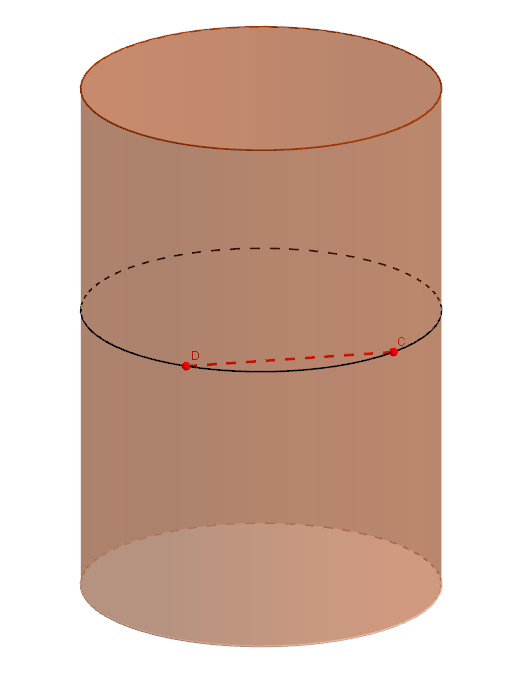
\includegraphics[width=0.3\columnwidth]{cilinderTwoPoints.png}
	 \label{fig:cube}
	\end{figure}
   \item O vértice A do triângulo ABC encontra-se sobre o semi-cículo BC. Assim
 podemos garantir que:
  
  \begin{enumerate}[a)]
    \item O triângulo é isóceles, porém pode não ser equilátero.
    \item O triângulo além de isóceles, é equilátero.
    \item O triângulo é retângulo.
    \item Área do setor ADE e os raios internos e externos AL e AD.
  \end{enumerate}
  
   \begin{figure}[H]
	 \centering
		\begin{tikzpicture}[line cap=round,line join=round,>=triangle 45,x=1.0cm,y=1.0cm]
		\clip(0.374,-3.712) rectangle (7.942,0.754);
		\fill[color=zzttqq,fill=zzttqq,fill opacity=0.1] (7.,-3.) -- (1.,-3.) -- (4.,0.) -- cycle;
		%\draw [shift={(4.,-3.)}] plot[domain=0.:π,variable=\t]({1.*3.*cos(\t
		% r)+0.*3.*sin(\t r)},{0.*3.*cos(\t r)+1.*3.*sin(\t r)}); 
		\draw [color=zzttqq] (7.,-3.)-- (1.,-3.);
		\draw [color=zzttqq] (1.,-3.)-- (4.,0.);
		\draw [color=zzttqq] (4.,0.)-- (7.,-3.);
		\begin{scriptsize}
		\draw [fill=qqqqff] (1.,-3.) circle (1.5pt);
		\draw[color=qqqqff] (0.594,-2.986) node {$B$};
		\draw [fill=qqqqff] (7.,-3.) circle (1.5pt);
		\draw[color=qqqqff] (7.304,-3.052) node {$C$};
		\draw [fill=uuuuuu] (4.,0.) circle (1.5pt);
		\draw[color=uuuuuu] (4.158,0.314) node {$A$};
		\end{scriptsize}
		\end{tikzpicture}
	\end{figure}
  \pagebreak[4]
  \item O padrão ISO 216 define o tamanho de formato de folhas retangulares como
  A4 e A5, ele determina que tanto A4 quanto A5 tem que possuir a mesma razão de
  proporção, ou seja, mesma razão entre o tamanho dos seus lados.
  Sabendo que na figura ABCD representa uma folha A4 e BCEF e AFED duas folhas
  A5 de mesmo tamanho, pois cada A4 é composta por exatamente duas A5. A
  razão de proporção da folha A4, é:
  
  \begin{enumerate}[a)]
    \item $1:\sqrt{2}$
    \item $1:\sqrt{3}$
    \item $1:2$
    \item $2:3$
  \end{enumerate}
  
  \begin{figure}[H]
  \centering
	  \begin{tikzpicture}[line cap=round,line join=round,>=triangle 45,x=1.0cm,y=1.0cm]
	\clip(5.58,-6.12) rectangle (12.5,1.98);
	\fill[color=zzttqq,fill=zzttqq,fill opacity=0.1] (7.02,0.98) -- (11.02,0.98) -- (11.02,-5.02) -- (7.02,-5.02) -- cycle;
	\draw [color=zzttqq] (7.02,0.98)-- (11.02,0.98);
	\draw [color=zzttqq] (11.02,0.98)-- (11.02,-5.02);
	\draw [color=zzttqq] (11.02,-5.02)-- (7.02,-5.02);
	\draw [color=zzttqq] (7.02,-5.02)-- (7.02,0.98);
	\draw [dash pattern=on 2pt off 2pt] (7.02,-2.02)-- (11.02,-2.02);
	\begin{scriptsize}
	\draw [fill=qqqqff] (7.02,-5.02) circle (1.5pt);
	\draw[color=qqqqff] (6.7,-5.34) node {$A$};
	\draw [fill=qqqqff] (7.02,0.98) circle (1.5pt);
	\draw[color=qqqqff] (6.66,1.4) node {$B$};
	\draw [fill=qqqqff] (11.02,0.98) circle (1.5pt);
	\draw[color=qqqqff] (11.18,1.52) node {$C$};
	\draw [fill=qqqqff] (11.02,-5.02) circle (1.5pt);
	\draw[color=qqqqff] (11.28,-5.38) node {$D$};
	\draw[color=zzttqq] (9.02,1.52) node {$b$};
	\draw[color=zzttqq] (5.88,-1.88) node {$a$};
	\draw [fill=uuuuuu] (11.02,-2.02) circle (1.5pt);
	\draw[color=uuuuuu] (11.16,-1.74) node {$E$};
	\draw [fill=uuuuuu] (7.02,-2.02) circle (1.5pt);
	\draw[color=uuuuuu] (6.88,-1.68) node {$F$};
	\end{scriptsize}
	\end{tikzpicture}
  
  \end{figure}
  
\end{enumerate}

\end{document}
